\documentclass[12pt]{article}
\usepackage[margin = 0.9in, top=0.8in]{geometry}
\usepackage{graphicx}
\usepackage{textgreek}
\usepackage{amsmath}
\usepackage{amsfonts}
\usepackage{mathtools}
\usepackage{amssymb}
\usepackage{float}
\usepackage{subcaption}
\usepackage{hyperref}
\usepackage{grffile}
\graphicspath{{./2/images},{./}}

\title{CS 754 - Advanced Image Processing\\Assignment 4 - Report}
\author{Shaan ul Haque - 180070053\\Mantri Krishna Sri Ipsit - 180070032}
\newcommand{\norm}[1]{\left\lVert #1 \right\rVert}
\newcommand{\R}{\mathbb{R}}
\begin{document}

\maketitle

\section*{Question 1}
\subsection*{1.a and 1.b}
We used ISTA to estimate the sparse vector. The final function is sum of cosines, impulses and noise. Thus, the final signal is not sparse in either DCT basis or the temporal basis. In order to overcome this problem, we create an over-complete the dictionary which is concatenation of 256×256 DCT matrix and 256×256 identity matrix column wise. We varied the sparsity level of the signal, in their respective sparse domain, and then for each sparsity level varied the standard deviation of the noise. We calculated maximum Eigenvalue for the dictionary to be used in ISTA algorithm while the hyper-parameter $\lambda$ was chosen to be 1 as we observed least overall RMSE in the reconstructed signal. Plot for the RMSE error for both the signal f1 and f2 is given below.  
\begin{figure}[H]
     \centering
     \begin{subfigure}[b]{0.47\textwidth}
         \centering
         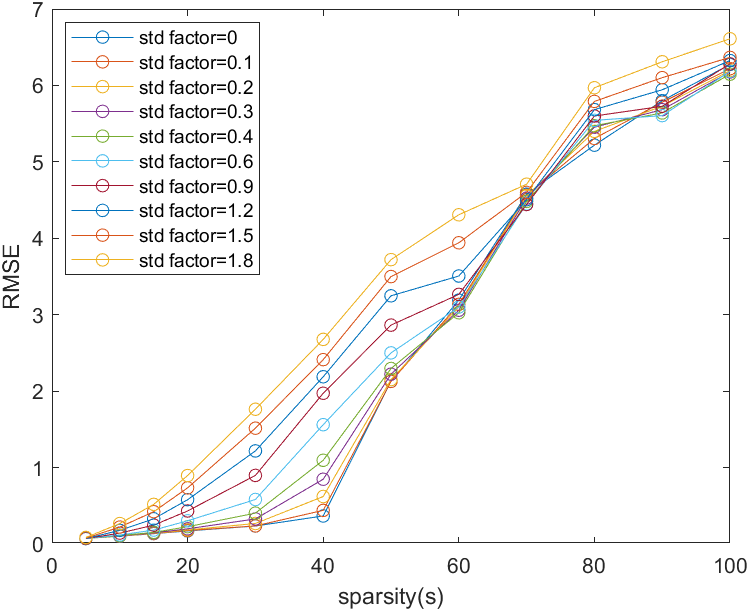
\includegraphics[width=\textwidth]{rmse_f1.png}
         \caption{$RMSE \ for \ f1$}
         \label{}
     \end{subfigure}
     \hfill
     \begin{subfigure}[b]{0.47\textwidth}
         \centering
         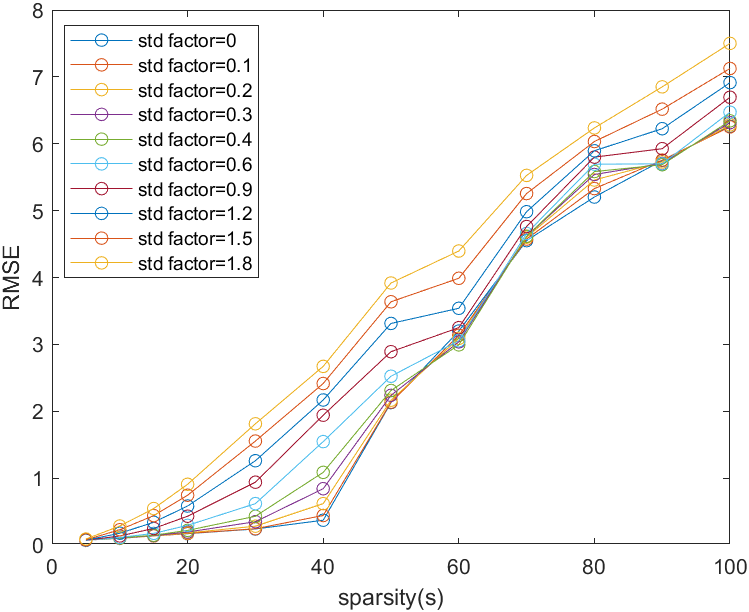
\includegraphics[width=\textwidth]{rmse_f2.png}
         \caption{$RMSE \ for \ f2$}
         \label{}
     \end{subfigure}
        \caption{RMSE}
        \label{fig:1}
\end{figure}
We observe that for same sparsity, increasing noise increases the RMSE error while increasing the sparsity level increases the noise as expected from the CS theorems. For large sparsity level(small S) typically in the range of 40 we observe that increasing noise has almost negligible effect on RMSE perhaps suggesting the small dependence of RMSE on noise variance (due to small S).
\subsection*{1.c}
We took sparsity level (s) = 20 and noise standard deviation factor = 0.5. We varied k from 0.1 to 10 in small steps initially and then larger steps subsequently. The figure shown below summarizes our result.
\begin{figure}[H]
  % will center the figure.
  \centering
  % include graphics (can include eps, jpg, pdf ...)
  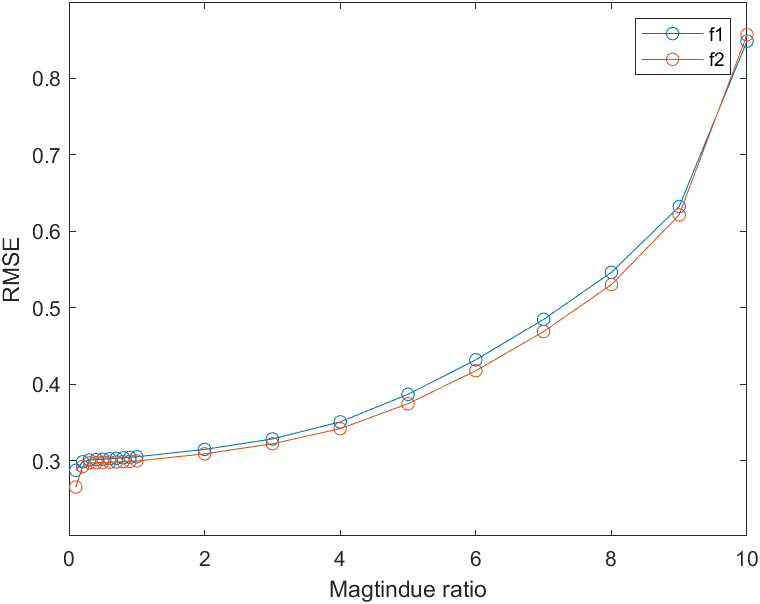
\includegraphics[scale=0.75]{assignment4/rmse_mag.png}  % change scale factor to re-size the image.
  % give a caption.
  \caption{RMSE vs k}
  % a label to refer to the figure
  \label{fig:2}
\end{figure}
We observe that as we increase K the RMSE increases which is as we should expect since noise standard deviation = 0.5(mean(f1)+mean(f2)), thus as magnitude of f2 is increased noise variance increases as well leading to larger RMSE. The hyper-parameter $\lambda$ was chosen to be 1.75 as we observed least overall RMSE for this value.

\section*{Question 3}
We know that by dictionary representation we can compactly express a large number image into small number of dictionary atoms. For any image, each of it's pixel value is the linear combination of those pixels in dictionary atom (when these atoms are represented into images by reshaping the columns). Due to this linearity, any linear operation done on the dictionary atoms gets reflected as it is in the image as well and vice versa. This can be seen from the following equations. \\
Let an image, $\boldsymbol{I} \in \boldsymbol{S}$, be represented by a linear combination of $s$ elements of a dictionary, given by $\boldsymbol{D} = \{\boldsymbol{d_1}, \boldsymbol{d_2}... \boldsymbol{d_k}\}$, that is the dictionary has total k atoms.
\begin{equation*}
    \boldsymbol{I} = \sum_{j=1}^{s} a_j\boldsymbol{d_{m_j}}  
\end{equation*}
where $a_j$ are the weights and $m_j$ are the column indices. If the dictionary atoms(columns) are reshaped into matrix, for each pixel in image we can observe that:
\begin{equation*}
    I(x,y) = \sum_{j=1}^{s} a_jd_{m_j}(x,y) \ \ \forall (x,y) \in \boldsymbol{I}
\end{equation*}
Let us perform any linear operation on the pixels of the image, mathematically:
\begin{equation*}
    f(I(x_l,y_l)) = \sum_{i=1}^{n}b_iI(x_{li},y_{li}) \ \ \forall (x_l,y_l) \in \boldsymbol{I}
\end{equation*}
where $(x_{li}, y_{li})$ are the spatial locations that the linear transformation takes into account (l and i will be related according to the linear transformation, for example $I(x_{li}, y_{li})$ might be the 8-neighborhood pixels around $(x_l, y_l)$, etc). Replacing $I(x_i, y_i)$, we get:
\begin{equation*}
    f(I(x_l,y_l)) = \sum_{i=1}^{n}b_i\sum_{j=1}^{s} a_jd_{m_j}(x_{li},y_{li})
\end{equation*}
Interchanging the summation:
\begin{equation*}
    f(I(x_l,y_l)) = \sum_{j=1}^{s}a_j(\sum_{i=1}^{n}b_i d_{m_j}(x_{li},y_{li}))
\end{equation*}
The term inside the brackets is the same linear operation albeit on the dictionary atoms. Thus we have shown that:
\begin{equation*}
    f(\sum_{j=1}^{s} a_jd_{m_j}(x,y)) = f(I(x_l,y_l)) = \sum_{i=1}^{s}a_jf(d_{m_j}(x_l,y_l)) 
\end{equation*}
\subsection*{3.a}
Any derivative filter on an image is a linear function of the pixels. Thus, as shown above, for the images in $\boldsymbol{S_1}$ the dictionary can be easily constructed using the  same derivative filter on the atoms of the $\boldsymbol{D}$ as used for the images in $\boldsymbol{S}$. Thus the newly formed dictionary will be $\boldsymbol{D_1} = \{f(\boldsymbol{d_1}), f(\boldsymbol{d_2})... f(\boldsymbol{d_k})\}$, where k is the number of dictionary atoms and \textit{f} is the derivative filter.
\subsection*{3.b}
Again, rotation of any image is linear transformation on the image pixels. But here we need slight tweaking in the sense there are two known angles, $\alpha$ and $\beta$, in which the images are rotated. Thus to overcome this issue we will rotate all the atoms (represented as images) by $\alpha$ and $\beta$ separately and then concatenated both the dictionaries column wise. The intuition behind this is same as we had for Question 1 of this assignment. If $\boldsymbol{D_{\alpha}} = \{\boldsymbol{d_{1\alpha}}, \boldsymbol{d_{2\alpha}}... \boldsymbol{d_{k\alpha}}\}$ and $\boldsymbol{D_{\beta}} = \{\boldsymbol{d_{1\beta}}, \boldsymbol{d_{2\beta}}... \boldsymbol{d_{k\beta}}\}$ represent rotated version of the columns (when represented in image form) then the final dictionary would be $\boldsymbol{D_{2}} = [\boldsymbol{D_{\alpha}} | \boldsymbol{D_{\beta}}]$.
\subsection*{3.c}
The given transformation is not linear in nature.
\begin{equation*}
    I_{new}(x,y) = \alpha(I_{old}(x,y))^2+\beta I_{old}(x,y)+\gamma
\end{equation*}
But we observe some pattern in the transformation which manifests itself in the dictionary as follows. Let the some image $\boldsymbol{I}\in \boldsymbol{S}$ be represented as:
\begin{equation*}
    \boldsymbol{I} = \sum_{j=1}^{s} a_j\boldsymbol{d_{m_j}}  
\end{equation*}
where the symbols have their usual meaning as defined earlier. Writing in pixel form we get:
\begin{equation*}
    I(x,y) = \sum_{j=1}^{s} a_jd_{m_j}(x,y) \ \ \forall (x,y) \in \boldsymbol{I}
\end{equation*}
Applying the quadratic transformation, we get:
\begin{equation*}
    I_{new}(x,y) = \alpha(\sum_{j=1}^{s} a_jd_{m_j}(x,y))^2+\beta(\sum_{j=1}^{s} a_jd_{m_j}(x,y))+\gamma 
\end{equation*}
Opening the square term, we get:
\begin{equation*}
    I_{new}(x,y) = \alpha(\sum_{j=1}^{s} a_j^2d_{m_j}^2(x,y)+2\sum_{i\not= j}a_ia_jd_{m_i}(x,y)d_{m_j}(x,y))+\beta(\sum_{j=1}^{s} a_jd_{m_j}(x,y))+\gamma 
\end{equation*}
Observing the above term, it is clear that the new dictionary must be concatenation of various functions of the dictionary columns. The new dictionary must have each column squared(element wise), pairwise product(element wise) of each column and a constant ones column(scaling will not matter as it will get absorbed in the coefficient). Thus new dictionary would be concatenation of:
\begin{equation*}
    \boldsymbol{D_{sq}} = \{\boldsymbol{d_1}^2, \boldsymbol{d_2}^2... \boldsymbol{d_k}^2\}
\end{equation*}
where $\boldsymbol{x}^2$ means element wise square of the vector. 
\begin{equation*}
    \boldsymbol{D_{pr}} = \{...\boldsymbol{d_i}\cdot\boldsymbol{d_j}...\} \ \ \forall i\not=j \ \ i,j\in \{1, 2, ... s\}
\end{equation*}
where $\boldsymbol{x\cdot y}$ means element wise product of the vectors.
\begin{equation*}
    \boldsymbol{D_c} = ones(\# \ of \ columns(D), 1)
\end{equation*}
Thus, $\boldsymbol{D_3} = [\boldsymbol{D_{sq}}| \boldsymbol{D_{pr}}| \boldsymbol{D}| \boldsymbol{D_c}]$

\subsection*{3.d}
Blur kernels are linear transformation on images only, such as the Gaussian blur filter. Thus as done for derivative filter, we can apply this known blur kernel to all the atoms of the dictionary(represented as images) to get the required dictionary. If \textit{f} is the known blur kernel, then the final dictionary $\boldsymbol{D_4} = \{f(\boldsymbol{d_1}), f(\boldsymbol{d_2})... f(\boldsymbol{d_k})\}$.
\subsection*{3.e}
Let the set of blur kernel $\boldsymbol{B} = \{\boldsymbol{b_1}, \boldsymbol{b_2}... \boldsymbol{b_p}\}$. Now let us pick any image $\boldsymbol{I_{blur}}$ from set $\boldsymbol{S_5}$ which is a blurred image of $\boldsymbol{I}$ from $\boldsymbol{S}$.
\begin{equation*}
    \boldsymbol{I_{blur}} = \sum_{i=1}^{n}c_i\boldsymbol{b_i(I)}
\end{equation*}
where $c_i$ is the weights for the blur kernel for the image. From part d, we know that blur kernel gets applied as it is to the atoms of the dictionary as well. Thus, all the new images in the set $\boldsymbol{S_5}$ are essentially linear combination of various blurred atoms from the dictionary with appropriate weights. The new dictionary will be concatenation of various blurred dictionary atoms, $\boldsymbol{D_5}$ = $[\boldsymbol{b_1(D)}| \boldsymbol{b_2(D)}|... \boldsymbol{b_p(D)}]$, where $\boldsymbol{b_i(D)} = \{\boldsymbol{b_i(d_1)}, \boldsymbol{b_i(d_2)}... \boldsymbol{b_i(d_k)}\}$, i.e., the blur kernel applied to all the atoms of the dictionary.

\end{document}
